\chapter{Prostorno hashiranje}
\label{chapter:spatial}

Prostorno hashiranje je metoda reprezentiranja trodimenzionalnog prostora u
jednodimenzionalnoj hash tablici. Temelji se na fiksnoj podjeli prostora na
\textit{AABB}-ove i raspodjelu istih tih \textit{AABB}-ova u čelije tablice (Slika \ref{figure:spatial}). ~\cite{gamedev}

\begin{figure}[h!]
    \centering
    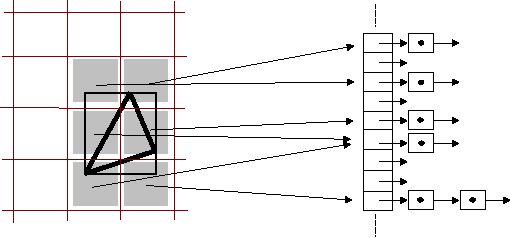
\includegraphics[width=12cm]{spatial.png}
    \caption {Pojednostavljeni 2D prikaz preslikavanja u hash tablicu.}
    \label{figure:spatial}
\end{figure}

\section{Priprema strukture za hashiranje}

Konstruktor hash tablice, kao i konstruktor \textit{Octree} strukture, kao argumente
prima mrežu trokuta od kojih je napravljen trodimenzionalni objekt, kao i željenu
dubinu podjele prostora. Za razliku od oktalnog stabla, kod prostornog hashiranja
prolazak kroz strukturu ne događa se rekurzivno, već su nakon prve rekurzivne podjele
prostora svi \textit{AABB}-ovi poznati.
Prostor se dijeli na \[n = 2^{(d\cdot l)}\] \textit{AABB}-ova.
Broj $d$ označava broj dimenzija, dok $l$ predstavlja koliko puta će se taj prostor
prepoloviti po svakoj svojoj dimenziji.\\
Na primjeru (Slika \ref{partitioning}):\\
Broj dimenzija $d$ je 2, a originalni \textit{AABB} smo odlučili prepoloviti dva puta, pa je rezultantni broj \textit{AABB}-ova 16 ($n = 2^{2*2}$)

\begin{figure}[h!]
    \centering
    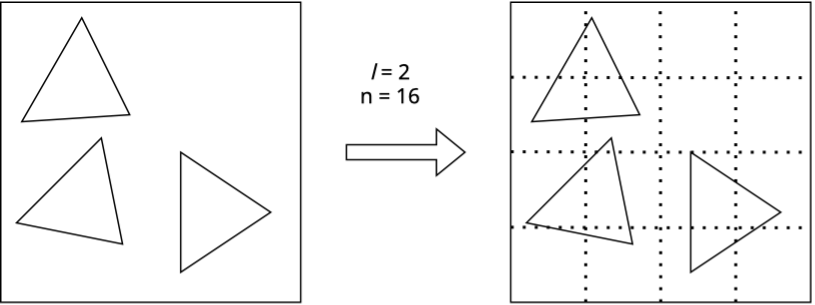
\includegraphics[width=12cm]{partitioning.png}
    \caption {Prikaz podjele prostora u dvije dimenzije}
    \label{partitioning}
\end{figure}

\begin{cppSource}{Implementacija funkcije za podjelu prostora}
std::vector<BoundingBox *>
BoundingBox::split(int level, const std::vector<Triangle> &triangles) {
    std::deque<BoundingBox *> queue;
    auto this_children = this->children();
    std::for_each(
        this_children.begin(),
        this_children.end(),
        [&queue, &triangles](BoundingBox *child) {
            queue.push_back(child);
            std::copy_if(
                triangles.begin(),
                triangles.end(),
                std::back_inserter(child->members()),
                [&child](const Triangle &triangle) {
                    return child->contains(triangle);
                }
            );
        }
    );

    while (queue.front()->level() != level) {
        std::array<BoundingBox *, 8> box_children = queue.front()->children();
        std::for_each(
            box_children.begin(),
            box_children.end(),
            [&queue](BoundingBox *child) {
                queue.push_back(child);
                std::copy_if(
                    queue.front()->members().begin(),
                    queue.front()->members().end(),
                    std::back_inserter(child->members()),
                    [&child](const Triangle &triangle) {
                        return child->contains(triangle);
                    }
                );
            }
        );
        queue.pop_front();
    }

    std::vector<BoundingBox *> retval(std::begin(queue), std::end(queue));

    return retval;
}
\end{cppSource}

\pagebreak
\section{Hash funkcija}

Hash funkcija koja se koristi kod prostornog hashiranja definirana je kao

\begin{equation}
    h = (\lfloor \frac{x}{k} \cdot P_1 \rfloor \oplus \lfloor \frac{y}{k} \cdot P_2 \rfloor \oplus \lfloor \frac{z}{k} \cdot P_2 \rfloor) \mod t
\end{equation}

gdje je \textit{t} veličina hash tablice, \textit{k} predefinirana
konstantna vrijednost, a $ P_{1..3} $ proizvoljno velik prost broj. ~\cite{spatialhashing}

\begin{cppSource}{Implementacija hash funkcije u jeziku C++}
int SpatialHashMap::_hash(BoundingBox* box) {
    Vertex center = box->center();

    return (static_cast<int>(center.x / CELL_SIZE * P1) ^
            static_cast<int>(center.y / CELL_SIZE * P2) ^
            static_cast<int>(center.z / CELL_SIZE * P3)) %
           TABLE_SIZE;
}
\end{cppSource}

\section{Stvaranje hash tablice}

Umetanje točaka u hash tablicu odvija se prema sljedećem algoritmu:

\begin{enumerate}
    \item Izračuna se hash vrijednost točke
    \item Ako u hash tablici već postoji ta vrijednost, točka se dodaje u \textit{vector}
    \item Ako vrijednost ne postoji, stvori se novi ključ te se inicijalizira \textit{vector}
          u kojeg se umetne ta točka
\end{enumerate}

Zbog jednostavnosti algoritma i optimizacije performansi, hash funkcija se ne
računa za svaki trokut mreže, već se \textit{hashiraju} samo središnje točke
\textit{AABB}-ova. Nakon što je poznata hash vrijednost središnje točke, u
hash tablicu se umeću svi trokuti koji pripadaju tom \textit{AABB}-u.


\begin{cppSource}{Umetanje \textit{AABB}-ova u hash tablicu}
void SpatialHashMap::insert(BoundingBox* box) {
    int hash = this->_hash(box);

    if (!box->members().size()) return;

    std::map<int, std::vector<Triangle>>::iterator cell = this->_map.find(hash);
    if (cell != this->_map.end()) {
        std::copy(
            box->members().begin(),
            box->members().end(),
            std::back_inserter(cell->second)
        );
        return;
    }

    this->_map.insert_or_assign(hash, box->members());
}
\end{cppSource}

\section{Algoritam za otkrivanje sudara}

Algoritam za otkrivanje sudara korištenjem hash
tablice izveden je sljedećim algoritmom:

\begin{enumerate}
    \item Objekt s kojim se želi provjeriti sudar podijeli se na jednak broj razina kao i 
          postojeći objekt u hash tablici
    \item Za svaki od \textit{AABB}-ova:
    \begin{enumerate}[i.]
        \item Izračuna se hash vrijednost
        \item Ako ta vrijednost postoji u hash tablici, provjeravaju
              se svi trokuti iz te čelije tablice
        \item Ako ta vrijednost ne postoji u tablici, prelazi se na sljedeći čvor
    \end{enumerate}
\end{enumerate}

\begin{cppSource}{Algoritam za otkrivanje sudara}
bool SpatialHashMap::collides(const std::vector<Triangle>& triangles) {
    std::vector<Vertex> vertices;

    for (const Triangle& triangle : triangles)
        std::for_each(
            triangle.begin(),
            triangle.end(),
            [&vertices](const Vertex& vertex) {
                vertices.push_back(vertex);
            }
        );

    BoundingBox root(vertices);
    std::vector<BoundingBox*> children = root.split(this->_levels, triangles);

    return std::any_of(children.begin(), children.end(), [&](BoundingBox* box) {
        int hash = this->_hash(box);

        auto cell = this->_map.find(hash);
        if (cell != this->_map.end()) {
            return helpers::primes_intersect({cell->second, box->members()});
        }

        return false;
    });
}
\end{cppSource}